\documentclass[12pt]{article}
 
\usepackage[margin=1in]{geometry} 
\usepackage{amsmath,amsthm,amssymb}
\usepackage{graphicx}
 
\newcommand{\N}{\mathbb{N}}
\newcommand{\Z}{\mathbb{Z}}
 
\newenvironment{theorem}[2][Theorem]{\begin{trivlist}
\item[\hskip \labelsep {\bfseries #1}\hskip \labelsep {\bfseries #2.}]}{\end{trivlist}}
\newenvironment{lemma}[2][Lemma]{\begin{trivlist}
\item[\hskip \labelsep {\bfseries #1}\hskip \labelsep {\bfseries #2.}]}{\end{trivlist}}
\newenvironment{exercise}[2][Exercise]{\begin{trivlist}
\item[\hskip \labelsep {\bfseries #1}\hskip \labelsep {\bfseries #2.}]}{\end{trivlist}}
\newenvironment{problem}[2][Problem]{\begin{trivlist}
\item[\hskip \labelsep {\bfseries #1}\hskip \labelsep {\bfseries #2.}]}{\end{trivlist}}
\newenvironment{question}[2][Question]{\begin{trivlist}
\item[\hskip \labelsep {\bfseries #1}\hskip \labelsep {\bfseries #2.}]}{\end{trivlist}}
\newenvironment{corollary}[2][Corollary]{\begin{trivlist}
\item[\hskip \labelsep {\bfseries #1}\hskip \labelsep {\bfseries #2.}]}{\end{trivlist}}

\newenvironment{solution}{\begin{proof}[Solution]}{\end{proof}}
 
\begin{document}
 
\title{Project 2: Gravitational Constant}
\date{Due July 3rd}

\maketitle

The purpose of this experiment is to illustrate a bit of physics and the application of statistics to estimating the gravitational constant. The gravitational constant will be estimated by rolling various objects down an incline. \\

\noindent
\textbf{Requirements:}

\begin{itemize}
	\item 4 objects to roll: marble, golf ball, racquetball, and toy car
	\item Tube constructed from poster board
	\item Pencil and paper
	\item Stop watch (phone)
	\item Calculator
	\item Protractor
	\item Yardstick or tape measure
\end{itemize}

\noindent
\textbf{Estimating the Gravitational Constant}

It is well known that the gravitational constant is 9.8 m/$\text{s}^2$. To be more precise, a body falling on Earth would accelerate at 9.8 m/$\text{s}^2$ without any friction. For the incline in the figure, Galileo stated the following relationship:

\begin{equation}
	a = g \sin{\theta}
\end{equation}

\noindent where $a$ is the acceleration, $g$ is the gravitational constant (9.8 m/$\text{s}^2$), and $\theta$ is the angle of the incline.

\begin{figure}[h]
	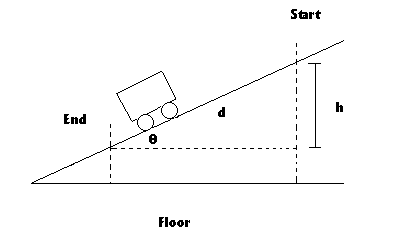
\includegraphics[scale=1]{incline}
\end{figure}

The basic procedure will be to set up an incline much like that above. The "Start" and "End" points will be the beginning and ending of the tube. The length of the tube will be the distance $d$. One student will hold an object with the leading edge of the object lined up with the start and will give a verbal signal while simultaneously releasing the car. At the signal, another student will start the stopwatch and will stop the stopwatch the instant the leading edge of the object reaches the end of the tube. The time on the stopwatch, $t$, will be recorded. With this information, we can estimate the gravitational constant as follows.

The quantity $h$ will be measured with the yardstick. Since the yardstick is in inches, the height will need to be converted to centimeters (and subsequently meters) using the conversion 1 inch equals 2.54 centimeters, or 1 inch equals 0.0254 meters. Since this forms a right triangle, we know that $\sin{\theta} = \frac{h}{d}$ (opposite divided by hypotenuse). Therefore the relationship given by Galileo can be rewritten as:

\begin{equation}
	a = g \cdot \frac{h}{d}
\end{equation}

\noindent From this we can solve for $g$ as

\begin{equation}
	g = a \cdot \frac{d}{h}
	\label{eq:g1}
\end{equation}

\noindent Acceleration, $a$, can be computed through the relationship

\begin{equation}
	d = v_0t + \frac{1}{2}at^2
\end{equation}

\noindent The quantity $v_0$ is the initial velocity, and is 0 in our experiments, so we can solve for $a$ as

\begin{equation}
	a = 2 \frac{d}{t^2}
\end{equation}

\noindent Plugging this into equation \ref{eq:g1} we get

\begin{equation}
	g = \frac{2d^2}{ht^2}
	\label{eq:g2}
\end{equation}

\newpage
\noindent
\textbf{Setting up the Design}

First, your group needs to brainstorm what factors would be of interest to study. That is, what factors might have an influence on what the value of $g$ would be estimated as. Some obvious ones are

\begin{enumerate}
	\item Student
	\item Type of object
	\item Length of tube ($d$)
	\item Angle/Height of tube (these are equivalent)
\end{enumerate}

\noindent Can you think of any more you would like to study? In this study, make sure you at least observe and record factors 2, 3, and 4. Feel free to study other factors.

After the factors have been decided on, the different values should be decided. For this study, factors 1, 2, and 3 are already set because the students and objects are known and the length of the tube is set. However, the angle of the tube can be anything and we can measure multiple angles. For this experiment, \textbf{use 2 separate angles for each object}. For each pairing of object and angle, \textbf{perform 5 trials.} You should have a total of 40 trials for the entire experiment.

Once the design is set up, put together a data sheet that will be used to record all of the data from all of the trials. Make sure there is a column to record the time and the estimated $g$, which will be computed using equation \ref{eq:g2}.

 Once the data has been collected, calculate the average gravitational constant for each group of factors (it will go quicker if each member of the group calculated the average for a given set of factors). Then discuss the following questions among with the members of your group:
 
 \begin{itemize}
 	\item How did the trials that were run agree with the true gravitational constant 9.8 m/$\text{s}^2$?
 	\item Based on your average calculations, which groups seemed to have different average value of the calculated gravitational constant?
 	\item If the groups seem to differ, what factors seem to be associated with the difference?
 	\item Are there outliers? Things you didn't expect? Things that concern you about the data?
 	\item What are other possible sources of variation in the data?
 \end{itemize}
 
\noindent \textbf{Write your answers to the above questions down and turn your data sheets and your answers. Turn in one sheet per group, ensuring all group member's names are on the sheet.}
 
\end{document}